\documentclass[conference,10pt]{IEEEtran}
\IEEEoverridecommandlockouts
\usepackage{graphicx,booktabs,amsmath,amssymb,xcolor,url,xspace,textcomp}
\usepackage[hidelinks]{hyperref}
\hypersetup{pdftitle={양팔 의류 조작을 위한 에고센트릭 인간 시연}, pdfauthor={Jeong Hwan Lee}}
\usepackage{array,tikz}
\usetikzlibrary{positioning,arrows.meta}
\usepackage{fontspec}\setmainfont{Times New Roman}\usepackage{xeCJK}\setCJKmainfont[AutoFakeBold=2.5]{AppleMyungjo}\setCJKsansfont[AutoFakeBold=2.5]{Apple SD Gothic Neo}\setCJKmonofont{Apple SD Gothic Neo}\xeCJKsetup{CJKecglue={},CJKspace=true}
\newcommand{\mm}{\,mm\xspace}
\def\UrlBreaks{\do\/\do\_\do\.\do\-}\def\UrlFont{\small\ttfamily}\newcommand{\code}[1]{\path{#1}}
\DeclareMathOperator*{\argmin}{arg\,min}
\definecolor{humF}{HTML}{E3F2FD}\definecolor{humS}{HTML}{1E88E5}
\definecolor{trjF}{HTML}{E8F5E9}\definecolor{trjS}{HTML}{43A047}
\definecolor{robF}{HTML}{FFEBEE}\definecolor{robS}{HTML}{E53935}
\definecolor{calF}{HTML}{FFFDE7}\definecolor{calS}{HTML}{F9A825}
\definecolor{senF}{HTML}{ECEFF1}\definecolor{senS}{HTML}{546E7A}
\definecolor{polF}{HTML}{F3E5F5}\definecolor{polS}{HTML}{8E24AA}
\renewcommand{\appendixname}{부록}

\begin{document}
\title{양팔 의류 조작을 위한\\에고센트릭 인간 시연:\\[1mm]\Large 손 착용 그리퍼 녹화에서 로봇 정책까지}
\author{\IEEEauthorblockN{Jeong Hwan Lee}
\IEEEauthorblockA{기술 보고서, 2026년 11월 2일 기준\\
저장소: \texttt{egocentric-garment-manipulation}}}
\maketitle

\begin{abstract}
우리는 원격 조작도, 로봇 데이터 수집도 없이 손 착용 그리퍼로 녹화한 인간 시연만으로 양팔 로봇이 티셔츠를 다루게 하려 한다.
시연자는 HandUMI 그리퍼 두 개(BrikHMP18의 오픈소스 설계이며 우리가 설계한 것이 아니다)를 착용하며, 각 그리퍼에는 피두셜
마커, 손목 어안 카메라, IMU, 그리고 2026년 10월 29일부터는 토크를 끈 엔코더로 읽는 집게 서보가 있다. 고정 RGB-D 카메라가 양손을
관찰한다. 모든 자세는 하나의 월드 좌표계, 즉 로봇 베이스로 표현되며, 이는 카메라--로봇 캘리브레이션(held-out 0.98\,px), 그
좌표계에서 측정한 시작점 마커, 캘리브레이션한 마커 리그(정적 오차 1--4\mm)로 정해진다. 모든 스트림은 하나의 호스트 시계를
공유한다. 집게 끝 자세는 고정 카메라의 점 추적(CoTracker3)을 마커로 고정하고 추적 공백에서만 IMU를 쓰는 방식으로 얻는다.
held-out 테이크에서 가린 마커 위치의 오차 중앙값은 16\mm(왼손), 19\mm(오른손)이며, 마커와 IMU 보간만 쓰면 약 42\mm{}이다. 손목
카메라 SLAM은 시도했으나 바로 잡는 순간에 추적을 잃어 기각했다. 데이터의 종단 간 시험으로, 먼저 변환한 시연을 reBot B601-DM 두
팔에서 개루프로 재생했다. 33\,s 시연 하나를 네 번 재생한 결과는 약 1\mm 이내로 반복되었고, 집게는 테이블 위 5--19\mm{}에서 닫혔으며
(사람은 약 10\mm), 로봇은 셔츠를 잡아 끌었지만 개지는 못했다. 이어서 정책 학습 데이터를 만들었다. 성공한 티셔츠 펴기 시연 300개를
시연 단위로 등급을 매기고, 라벨은 역기구학 \emph{이전}의 값을 클램프 없이 쓴다. 파인튜닝한 첫 정책들은 횟수를 세지 않은 로봇
시행에서 천에 닿기 전에 멈추고 집게를 일찍 닫았다. 기록된 원인은 두 가지(정책이 입력의 집게 상태를 그대로 따라 함, 로봇 손목
카메라 위치가 손 착용 집게와 다름)이고, 라벨을 점검해 데이터 문제 세 가지를 더 찾았다(라벨 클램프, 시연 속도, 영상 집게 라벨).
범위를 줄인 실현 가능성 시험(왼손으로 소매 하나 집기)에서는 시연 197개로 파인튜닝한 정책이 2026년 11월 2일 실제 로봇 시행에서
소매를 잡았다. 시행 횟수는 세지 않았고, 놓친 뒤에는 다시 시도하지 않고 다른 곳을 잡는다. 성공률은 보고하지 않는다.
\end{abstract}

% =====================================================================
\section{서론}\label{sec:intro}
티셔츠 개기는 긴 호흡의 양팔 접촉 작업이며, 잡을 때마다 천의 상태가 바뀐다. 이런 작업의 원격 조작 로봇 데이터는 모으기 느리고
비싸다. UMI~\cite{chi2024umi} 방식의 손에 드는 그리퍼와 손에 끼는 그리퍼는 로봇과 닮은 말단 장치로, 로봇 없이 사람이 시연하게
해 주므로 데이터 수집이 로봇 수가 아니라 사람 수에 비례해 늘어난다. 어려움은 변환으로 옮겨 간다. 캘리브레이션, 자세 복원, 집게
라벨링, 시간 맞춤, 기구학적 실현 가능성의 모든 오차가 학습 라벨에 들어가고, 그 라벨로 학습한 정책이 이를 물려받는다. 정책
성공률은 이런 오차에 대한 늦고 간접적인 신호다.

\textbf{주요 질문.} \emph{로봇이 변환된 인간 동작을 개루프로 그대로 재생하면, 사람이 한 일을 하는가?} 재생은 모든 단계
(캘리브레이션, 자세, 집게 상태, 로봇화, IK, 시간, 제어)를 한 번에 시험하고, 사람·로봇 명령·측정된 로봇 동작을 하나의 시계와
하나의 좌표계에 놓아 오차를 단계별로 나눌 수 있게 하며, 눈에 보이게 실패한다. 후속 질문은 같은 변환이 정책이 잡기를 배울 수 있는
라벨을 만드는가이다.

\textbf{지금까지의 기여:}
\begin{itemize}
\item 캘리브레이션과 시작점 마커로 한 번 정하는 하나의 월드 좌표계(로봇 베이스). 사람과 로봇의 경로가 테이크별 정렬 없이 이를
  공유한다(\ref{sec:cal}절);
\item 잡는 순간에도 유지되는 손 착용 그리퍼의 자세 소스: 피두셜 마커로 고정한 고정 카메라 점 추적, 공백에서만 IMU, held-out
  마커로 검증(\ref{sec:pose}절); 서보 엔코더에서 얻는 집게 라벨(\ref{sec:jaw}절);
\item 사람·명령·로봇을 하나의 시계로 비교하는 개루프 재생 시험과 그 측정 결과(\ref{sec:replay}절);
\item 시연별 등급과 IK 이전 데카르트 라벨을 쓰는 학습 데이터 파이프라인, 로봇에서의 첫 정책들, 기록된 실패 원인과 그 뒤
  찾은 데이터 문제(\ref{sec:data}--\ref{sec:policy}절).
\end{itemize}

\textbf{현황}(2026년 11월 2일). 재생은 끝났고, 재생으로 개기는 성공하지 못한다. 펴기 데이터로 파인튜닝한 정책은 횟수를 세지 않은
로봇 시행에서 잡지 못했다. 소매 하나 집기 시험(\ref{sec:pinch}절)에서는 11월 2일 실제 로봇 시행에서 잡기에 성공하는 것이
관찰되었다. 시행 횟수는 세지 않았다. 횟수를
센 시행을 하지 않았으므로 이 보고서 어디에서도 성공률은 보고하지 않는다.

\textbf{이전 버전과의 관계.} 이 보고서는 재생 트랙을 자세히 다룬 버전 0.1(10월 27일)과 버전 0(10월 21일), 그리고 짧은 기술 노트를
대체한다. 이전 문서들은 \code{report/archive/}에 있다. 현재 파이프라인에 더는 영향을 주지 않는 재생 시기의 세부 내용은 여기서
뺐고, 대체된 방법은 표~\ref{tab:superseded}에 정리했다.

\begin{figure}[!t]
\centering
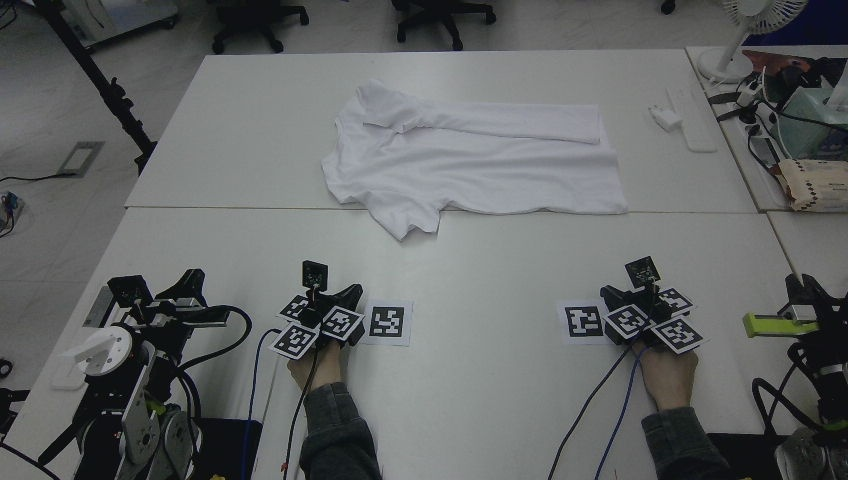
\includegraphics[width=\columnwidth]{figures/fig_scene.jpg}
\caption{고정 RGB-D 카메라에서 본 셋업: 테이블 위 티셔츠, 피두셜 마커가 붙은 시연자의 손 착용 그리퍼 두 개가 시작점 마커 두 개
위에 놓여 있고, 로봇 팔 두 개가 왼쪽과 오른쪽 가장자리에 있다.}
\label{fig:scene}
\end{figure}

% =====================================================================
\section{관련 연구}\label{sec:related}
\textbf{손에 드는/끼는 그리퍼.} UMI~\cite{chi2024umi}는 평행 집게 그리퍼와 손목 어안 카메라로 시연을 녹화하며, 자세는
ORB-SLAM3~\cite{campos2021orbslam3} 기반 단안-관성 SLAM에서 얻고, 궤적은 대상 로봇의 기구학으로 거른다.
HandUMI~\cite{handumi,meza2026handumi}는 BrikHMP18과 공동 저자들이 설계·공개한 로봇 없는 양팔 데이터 수집용 손 착용형
오픈소스 변형이며, 우리는 그 빌드 사본을 쓴다. DexUMI~\cite{xu2025dexumi}는 외골격을 낀 사람 손을 정교한 로봇 손의 인터페이스로
쓴다. 우리는 UMI 방식 그리퍼는 유지하되 자세를 손목 SLAM이 아닌 고정 RGB-D 카메라에서 얻고, 정책 학습 전에 대상 로봇에서 데이터를
시험한다. 실현 불가능한 궤적을 제거하는 대신, 사람의 경로를 라벨로 유지하고 실현 가능성은 실행기에 맡긴다.

\textbf{인간 데이터와 저가 양팔 로봇.} EgoMimic~\cite{kareer2025egomimic}은 에고센트릭 인간 영상과 로봇 데이터를 함께 학습한다.
ALOHA~\cite{zhao2023aloha}는 저가 팔과 원격 조작으로 세밀한 양팔 조작을 보였다. 우리는 저가 reBot B601-DM 두 팔을
LeRobot~\cite{cadene2024lerobot}으로 쓰되, 원격 조작 없이 녹화한다.

\textbf{천.} 의류 개기와 펴기는 전용 프리미티브로 학습되어 왔다(예: SpeedFolding~\cite{avigal2022speedfolding},
FlingBot~\cite{ha2021flingbot}). 우리는 천 전용 방법을 제안하지 않으며, 정책은 일반적인 디퓨전 트랜스포머~\cite{peebles2023dit}와
VLA~\cite{xvla}이다.

\textbf{자세, 캘리브레이션, 기구학.} 마커는 AprilTag~\cite{olson2011apriltag,wang2016apriltag2}이며 OpenCV~\cite{bradski2000opencv}로
검출하고 IPPE~\cite{collins2014ippe}와 SQPnP~\cite{terzakis2020sqpnp}로 푼다. 점 추적은 CoTracker3~\cite{karaev2024cotracker3},
회전은 Mahony 필터~\cite{mahony2008ahrs}를 쓴다. 카메라--로봇 풀이는 Shah의 방법~\cite{shah2013robotworld}으로 초기화한다. IK는
Pinocchio~\cite{carpentier2019pinocchio} 위의 Pink~\cite{pink}를 쓴다. 자세 소스로 평가했다가 기각한 것: MASt3R-SLAM~\cite{murai2025mast3rslam},
ORB-SLAM3, 그리고 이전 스테레오 카메라에서의 Basalt~\cite{usenko2020basalt}, OpenVINS~\cite{geneva2020openvins},
AirSLAM~\cite{xu2025airslam}.

% =====================================================================
\section{시스템 개요}\label{sec:overview}
\begin{figure*}[!t]
\centering
\begin{tikzpicture}[font=\scriptsize, node distance=4mm and 5mm,
  arr/.style={-{Latex[length=1.8mm]},thick},
  darr/.style={-{Latex[length=1.6mm]},dashed,semithick},
  box/.style={draw=#1S, fill=#1F, rounded corners=3pt, line width=0.8pt, text width=27mm, minimum height=12mm,
    align=center, inner sep=2pt}]
\node[box=cal] (cal) {\textbf{하나의 월드 좌표계}\\카메라 $\to$ 로봇 베이스; 시작점 마커; 마커 리그 $\to$ 집게 끝};
\node[box=hum, right=of cal] (pt) {\textbf{점 추적}\\CoTracker3 점을 깊이로 들어 올림, 강체 피팅, 게이트};
\node[box=hum, right=of pt] (fu) {\textbf{자세 융합 (Cg)}\\마커가 추적을 고정; IMU는 공백에서만};
\node[box=hum, right=of fu] (jw) {\textbf{집게 라벨}\\서보(새 시연) 또는 영상 모델(이전 시연), 섞지 않음};
\node[box=trj, right=of jw] (gr) {\textbf{에피소드}\\대기·가장자리 트림; GOLD / SILVER / REJECT};
\node[box=sen, above=of pt] (orb) {\textbf{고정 RGB-D 카메라}\\마커, 깊이, 장면};
\node[box=sen, above=of fu] (imu) {\textbf{손목 IMU}\\자이로 + 가속도계};
\node[box=sen, above=of jw] (srv) {\textbf{집게 서보}\\토크 끔, 엔코더로 읽음};
\node[box=sen, above=of gr] (fis) {\textbf{손목 어안 카메라}\\집게, 주변 천};
\node[box=trj, below=of gr] (lb) {\textbf{라벨}\\IK 이전의 융합 집게 끝, 클램프 없음; 시간 늘린 사본};
\node[box=pol, left=of lb] (po) {\textbf{정책}\\공개 천 데이터로 사전학습, 우리 시연으로 파인튜닝};
\node[box=rob, left=of po] (dp) {\textbf{로봇}\\FK $\to$ 청크 $\to$ 제한기 $\to$ IK $\to$ 안전; 재계획};
\node[box=rob, dashed, left=of dp, text width=45mm] (rp) {\textbf{재생 트랙(완료)}\\로봇화 $\to$ 한계 고려 IK $\to$ 개루프 재생 $\to$ 사람 / 명령 / 로봇 비교};
\draw[arr] (orb) -- (pt); \draw[arr] (pt) -- (fu); \draw[arr] (imu) -- (fu);
\draw[arr] (srv) -- (jw); \draw[darr] (fis) -- (jw.north east);
\draw[darr,draw=calS] (cal) -- (pt);
\draw[arr] (fu) -- (jw); \draw[arr] (jw) -- (gr); \draw[arr] (gr) -- (lb); \draw[arr] (lb) -- (po);
\draw[arr] (po) -- (dp); \draw[darr] (fu.south) -- (rp.north east);
\end{tikzpicture}
\caption{2026년 11월 1일 기준 데이터 흐름. 회색: 센서, 모두 하나의 호스트 시계로 시각을 찍는다. 노란색: 사람과 로봇을 하나의
월드 좌표계에 놓는 한 번의 셋업. 파란색: 각 그리퍼의 자세와 집게 상태. 초록색: 등급을 매긴 에피소드와 학습 라벨. 보라색과
빨간색: 로봇에서의 정책과 실행. 점선 상자: 정책 학습 전에 변환을 시험한 개루프 재생 트랙(\ref{sec:replay}절). 손목 영상은 정책
입력이며, 서보를 다시 달기 전에 녹화한 시연에서만 집게 라벨을 제공한다.}
\label{fig:pipe}
\end{figure*}

그림~\ref{fig:pipe}는 현재 데이터 흐름이다. 두 원칙이 전체를 관통한다. \emph{하나의 월드 좌표계}: 사람이든 로봇이든 모든 자세를
로봇 베이스 좌표계로 표현하므로, 녹화별 정렬(SLAM 맵, 점군 정합)이 필요 없다. \emph{하나의 시계}: 카메라 프레임, IMU와 서보
샘플, 로봇의 명령·측정 관절이 모두 호스트 타임스탬프를 가지므로, 동기화 하드웨어 없이 사람·명령·로봇을 샘플 단위로 비교하고
같은 카메라로 나란히 촬영할 수 있다.

% =====================================================================
\section{하드웨어}\label{sec:hw}
\begin{table}[t]
\caption{구성 요소}\label{tab:hw}
\centering\small
\begin{tabular}{@{}>{\raggedright\arraybackslash}p{0.27\columnwidth}>{\raggedright\arraybackslash}p{0.65\columnwidth}@{}}
\toprule
장치 & 모델, 역할 \\
\midrule
손 착용 그리퍼 $\times$2 & HandUMI~\cite{handumi}, BrikHMP18 설계(우리 설계 아님), 우리 빌드; 시연 도구 \\
마커 & 그리퍼당 48\mm AprilTag 세 장, 10월 23일부터 손목 카메라 뒷면에 30\mm 태그 한 장 추가 \\
손목 카메라 $\times$2 & 어안, 1280$\times$720, 30\,Hz; 집게와 주변 천 \\
손목 IMU $\times$2 & Seeed XIAO nRF52840 Sense; 자이로와 가속도계 \\
집게 서보 $\times$2 & Feetech STS3215, 토크 끔, 호스트 시계로 약 100\,Hz 읽음(10월 13--28일 제거, 10월 29일부터 다시 장착) \\
RGB-D 카메라 & Orbbec Gemini 336, 컬러 + 정렬된 깊이(녹화 스트림 약 15\,Hz), 테이블 위 고정; 10월 25일 113\,cm로 올림(11월 1일 각도만 다시 맞춘 뒤 높이는 다시 재지 않음) \\
로봇 팔 $\times$2 & reBot B601-DM, 6-DoF + 평행 집게, USB-CAN의 Damiao 모터, 우리의 MIT 모드 브리지 100\,Hz \\
호스트 & Apple 실리콘 노트북: 녹화, IK, 브리지, 배포 루프 \\
GPU & 점 추적·집게 모델·3-D 풀이와 일부 정책 학습용 임대 RTX 5090 포드; 임대 H100에서 한 번 학습; DiT 파인튜닝용 Ray 경유 RTX 4090 \\
\bottomrule
\end{tabular}
\end{table}

\begin{figure}[!t]
\centering
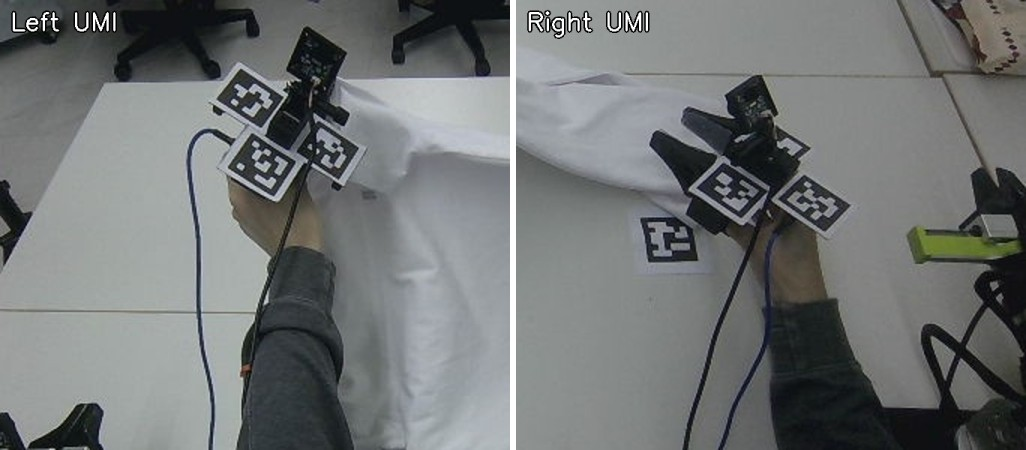
\includegraphics[width=\columnwidth]{figures/fig_umi.jpg}
\caption{10월 23일 이전에 녹화한 손 착용 그리퍼 두 개: 손마다 48\mm AprilTag 세 장, 손목 어안 카메라, IMU가 달린 HandUMI(BrikHMP18의
설계). 이 기간에는 집게 서보가 없었다. 10월 23일부터 손목 카메라 뒷면에 30\mm 태그가 하나 더 있고, 10월 29일부터 집게 서보가
엔코더로 다시 달려 있다.}
\label{fig:umi}
\end{figure}

표~\ref{tab:hw}에 구성 요소를 정리했다.

\textbf{HandUMI는 우리가 설계한 것이 아니다.} BrikHMP18이 설계·공개했으며(murobotics-ai,
\url{https://github.com/murobotics-ai/handumi-hw}, Apache-2.0)~\cite{handumi,meza2026handumi}, UMI~\cite{chi2024umi}를 따른다.
우리는 업스트림 부품(커밋 \texttt{e58de33})을 출력했고 다음을 바꾸었다(그림~\ref{fig:umi}): VR 추적 대신 손목 IMU; 컨트롤러 지지
커넥터, 카메라 마운트, 서보 커버 수정; 손마다 서로 다른 면에 AprilTag 여러 장을 붙여 적어도 한 장은 고정 카메라를 향하도록 했고,
10월 23일부터 손목 카메라 뒷면에 작은 태그를 추가했다. 이 태그 한 장만 보일 때의 평면 자세 뒤집힘은 IMU로 해소한다.

\textbf{집게 서보 이력.} 서보 축이 부러지고 장치가 무거워서 10월 13일에 집게 서보를 떼어 냈고, 10월 13일부터 28일까지는 집게 상태를
손목 영상에서 추정했다. 10월 29일에 서보를 다시 달았는데, 사람이 잡고 있을 때 집게를 구동하지 않도록 토크를 끄고 집게 열림의
엔코더로만 읽는다(\ref{sec:jaw}절).

\textbf{로봇.} reBot B601-DM 두 팔(제조사 LeRobot 플러그인과 URDF는 저장소에 없다)을 우리의 HTTP 브리지가 MIT 모드로 구동한다.
100\,Hz 스레드 하나, 목표를 향한 가속도 제한 동작, 스트리밍 명령 사이의 목표 보간, 꺼진 모터의 자동 재활성화, USB 재연결, 집게
열림 한계 강제. 브리지는 적분 항만 쓰는 피드포워드 토크를 쓰고 중력 모델이 없다. 이것이 추적 오차를 결정한 이유는
\ref{sec:replay}절에서 설명한다.

% =====================================================================
\section{하나의 월드 좌표계와 캘리브레이션}\label{sec:cal}
\begin{figure*}[!t]
\centering
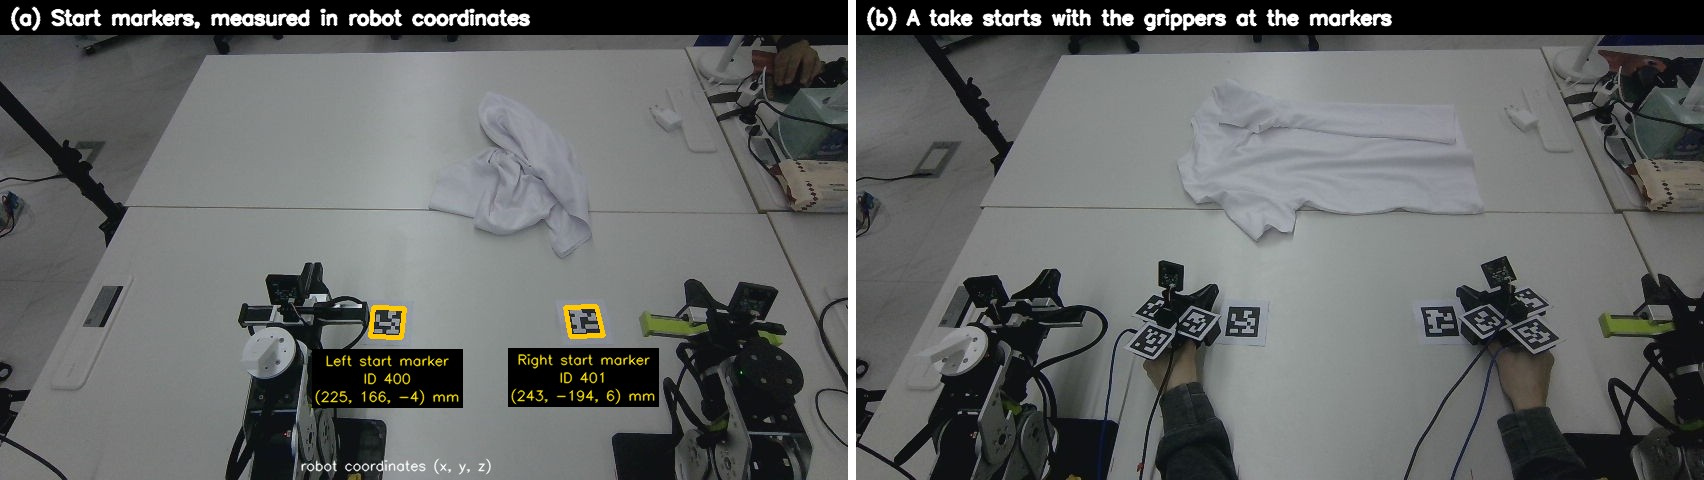
\includegraphics[width=0.85\textwidth]{figures/fig_start_markers.jpg}
\caption{시작점 마커. (a) 테이블에 붙인 AprilTag 두 장(ID 400 왼쪽, 401 오른쪽)을 캘리브레이션한 고정 카메라로 한 번 측정했고,
로봇 좌표계에서의 중심을 표시했다. (b) 모든 테이크는 두 그리퍼를 이 마커 위에 두고 시작하므로, 각 시연은 알려진 로봇 좌표에서
시작한다.}
\label{fig:start}
\end{figure*}

사람과 로봇 데이터는 하나의 월드 좌표계 $B$, 즉 로봇 베이스 좌표계($+x$ 앞, $+y$ 왼쪽, $+z$ 위)를 쓴다. 집게 끝 TCP는 두 집게
끝의 중점이며, 사람 그리퍼와 로봇 그리퍼에서 같은 방식으로 정의한다. $T_{XY}\in SE(3)$는 좌표계 $Y$의 좌표를 $X$로 옮긴다.
좌표계는 네 단계로 정한다.
\begin{enumerate}
\item \emph{카메라에서 로봇으로.} 첫 캘리브레이션: 로봇이 손목의 마커를 고정 카메라 앞에서 32개 자세로 유지한다. 미지수
  $T_{CB}$와 마커--TCP 변환은 $T_{C,m}(k)=T_{CB}\,T_{BE}(q_k)\,T_{E,m}$을 만족하며, Shah의 방법~\cite{shah2013robotworld}으로
  초기화하고 모든 태그 꼭짓점의 재투영과 깊이 잔차로 다듬는다(32개 중 18개 자세 사용, 5겹 held-out 검증). 펴기 테이크를 위해
  카메라를 옮겼고(96$\to$105$\to$113\,cm로 올림), 옮길 때마다 로봇을 움직이지 않고 $T_{CB}$를 다시 푼다. 로봇 좌표를 아는 테이블
  고정 70\mm 태그 두 장이 위치와 요를, 깊이 영상의 테이블 평면이 기울기와 높이를 정한다(\code{robot_cam_v002}--\code{v005}).
\item \emph{시작점 마커.} 두 시작점 마커를 캘리브레이션한 카메라로 한 번 측정한다(그림~\ref{fig:start}a, 표~\ref{tab:cal}).
\item \emph{마커 리그에서 집게 끝으로.} 천천히 돌리는 테이크로 각 그리퍼 리그의 태그 간 변환을 구하고, 리그 좌표계에서의 집게 끝
  오프셋 $t_\mathrm{tcp}$는 형상을 아는 보드의 꼭짓점을 짚어 얻는다:
  $t_\mathrm{tcp}=\argmin_t\sum_j\rho(\lVert p_{B,\mathrm{rig}}(j)+R_{B,\mathrm{rig}}(j)\,t-c_B(j)\rVert)$, $\rho$는 Huber 손실.
  피벗 테이크가 독립적인 확인을 준다.
\item \emph{모든 테이크의 시작.} 각 테이크는 그리퍼를 시작점 마커 위에 두고 시작한다(그림~\ref{fig:start}b).
\end{enumerate}

\textbf{현실에서 측정한 로봇 모델 보정.} 로봇 모델의 오차 세 가지는 실제 로봇을 줄자와 카메라로 재서야 발견되었다. URDF의 그리퍼
TCP가 실제 집게 끝보다 89\mm 앞에 있었고, 왼팔 베이스가 URDF보다 70\mm 안쪽에 3$^\circ$ 기울어 있었으며, 왼팔 두 번째 관절에
$-8.4^\circ$의 영점 오프셋이 있었다. 세 가지 모두 IK 모델 안에서 덮어쓰기로 적용하고(\code{configs/robot/}), URDF 파일은 건드리지
않는다. 모델을 모델 자신과 비교하는 FK 기반 일치도 검사로는 보이지 않았다.

\begin{table}[t]
\caption{캘리브레이션 결과}\label{tab:cal}
\centering\small
\begin{tabular}{@{}>{\raggedright\arraybackslash}p{0.40\columnwidth}>{\raggedright\arraybackslash}p{0.52\columnwidth}@{}}
\toprule
항목 & 결과 \\
\midrule
카메라 $\leftrightarrow$ 로봇 베이스 & held-out 재투영 0.98\,px, 측면 $\approx$1.3\mm \\
보정한 로봇 모델, 집게 절대 위치 & 홈 자세에서 줄자 측정과 6--9\mm 이내 \\
시작점 마커 400 / 401 & $(225, 166, -4)$\mm, $(243, -194, 6)$\mm \\
마커 리그 $\to$ 집게 끝 & 정적 1--4\mm; leave-one-out 1.8--4.8\mm; 독립 피벗 시험 RMS 5--7\mm \\
사람 $\leftrightarrow$ 로봇 그리퍼 방향 & 분산 2--9$^\circ$ \\
\bottomrule
\end{tabular}
\end{table}

% =====================================================================
\section{손 착용 그리퍼의 자세}\label{sec:pose}
\subsection{마커}
고정 카메라의 각 프레임에서 AprilTag를 검출하고 각각을 IPPE로 푼다. 한 변이 18\,px보다 작은 태그는 무시한다. 약 1\,m 거리에서
PnP의 가장 부정확한 좌표인 마커 거리는, 태그 안 깊이 중앙값이 PnP 값과 0.10\,m 이내이면 정렬된 깊이로 시선 방향을 따라 보정한다.
한 리그의 태그가 두 장 이상 보이면 모든 꼭짓점을 함께 풀고(SQPnP 후 Levenberg--Marquardt), 재투영 RMSE가 2\,px를 넘는 프레임은
버린다. 리그 자세, 집게 끝 오프셋, $T_{BC}$로 $B$에서의 집게 끝 자세를 바로 얻는다.

\subsection{마커로 고정한 점 추적(변형 Cg)}
천, 손바닥, 다른 손이 마커를 가릴 때마다 마커는 보이지 않으며, 이는 정확히 잡는 순간이다. 그래서 위치는 고정 카메라의 점 추적에서
얻고 마커를 앵커로 쓴다.
\begin{enumerate}
\item \emph{점.} CoTracker3(온라인 모드)가 그리퍼마다 질의점 40개를 컬러 영상에서 따라가며, 각 시연 시작 시 그리퍼 몸체에 심는다.
\item \emph{3-D.} 정렬된 깊이로 점을 3-D로 들어 올리고, 강체 그리퍼 모델을 맞춰 프레임별 그리퍼 몸체를 얻는다.
\item \emph{게이트.} 추적 가속도가 IMU 가속도와 맞지 않거나(1\,s 창에서 정규화 상호상관 $<0.2$, 보이는 태그가 추적과 일치하면
  예외), 두 손이 8\,cm보다 가까워지거나, 1\,s 안에 적어도 3 프레임에서 보이는 태그가 추적에서 10\,cm 넘게 떨어지면 그 프레임은
  무효이다.
\item \emph{융합.} 시연마다 20\,Hz 격자 위의 희소 최소제곱 문제 하나(Cauchy 가중): 유효한 추적점, 보이는 곳의 태그, 일정한 3-D
  편향, 2차 차분 평활 사전, 그리고 다른 지지가 없는 노드에\emph{만} IMU 가속도. 회전은 정지 구간에서 자이로 편향을 취하고 태그가
  두 장 이상 보이는 첫 프레임에 요를 고정한 Mahony 필터에서 얻는다.
\end{enumerate}

\textbf{정확도.} 실제로 보였던 마커를 가리고 추정값과 비교해 정확도를 잰다. 가린 실행에서는 어떤 것(요 앵커, 태그 인자, 편향)도
가린 태그에서 추정하지 않는다. 튜닝에 쓰지 않은 held-out 테이크에서 가린 마커 오차의 중앙값은 \textbf{16\mm(왼손), 19\mm(오른손)}이며,
마커와 IMU 보간만으로는 약 42\mm{}이다. 개발용 테이크에서 마커는 절대 오차를 42에서 12\mm{}로 줄였고, IMU 가속도를 모든 곳에 넣으면
결과가 나빠져서 IMU는 공백 안에서만 쓴다. 한 GOLD 펴기 시연에서 왼손은 프레임의 48\,\%에서 마커, 49\,\%에서 점 추적만, 3\,\%에서
IMU였고, 오른손은 77 / 23 / 0\,\%였다. 모든 시연에 QA 영상을 만든다(그림~\ref{fig:fusqa}).

\begin{figure*}[!t]
\centering
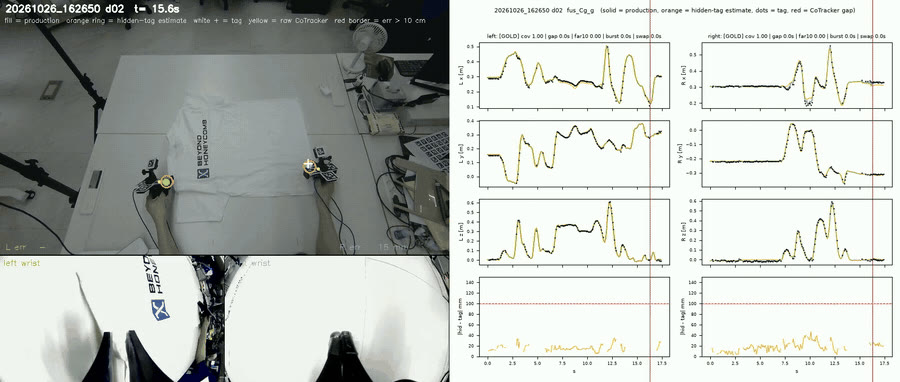
\includegraphics[width=0.85\textwidth]{figures/fig_fusion_qa.jpg}
\caption{GOLD 펴기 시연의 시연별 QA 영상. 왼쪽 위: 융합한 집게 끝(채운 점), 그 마커를 가리고 만든 추정(주황 고리), 마커 자체(흰 +),
CoTracker 원시 점(노랑)을 얹은 고정 카메라. 왼쪽 아래: 두 손목 카메라. 오른쪽: 손별 $x$, $y$, $z$의 시간 변화와 가린 마커 오차
(맨 아래 줄, 빨간 점선 = 10\,cm).}
\label{fig:fusqa}
\end{figure*}

\subsection{이전에 시도한 것과 실패한 이유}\label{sec:slam}
Cg 이전에 세 가지 자세 소스를 시도했다. (i) \emph{손목 카메라 SLAM.} 추적을 잃으면 자동으로 재시작하는 손목 어안 MASt3R-SLAM은
추적하는 곳에서는 정확했지만(held-out 마커 프레임에서 2--14\mm), 프레임의 19--48\,\%, 잡는 순간 주변 마커가 가려진 프레임의
0--38\,\%만 남겼고, 재시작한 구간 사이의 이음새는 40--73\mm 튀었다. 가까운 거리에서 흰 천이 시야를 채우고 손이 빠르게 움직이기
때문이다. ORB-SLAM3 단안-관성은 좋은 회전으로 초기화되었지만 이동 스케일이 30--1000$\times$로 발산했다. 손의 가속도(중앙값
0.07--0.16\,m/s$^2$)가 가속도계 편향(0.25--0.43\,m/s$^2$)보다 작아 스케일을 관측할 수 없었다. 이전 스테레오 카메라의 스테레오
VIO도 발산했고, 그 카메라는 10월 16일에 뺐다. (ii) \emph{이전 평활기}(SLAM + 외부 몸체 추적 + IMU)는 자체 품질 검사를 모두
통과했지만 외부 카메라가 본 집게 위치와 4--6\,cm 떨어져 있었다. 오래된 카메라--IMU 회전(17--24$^\circ$ 어긋남), 20--35\,cm
잘못 수렴한 레버 암, 잘못된 앵커 때문이었고, 내부 잔차로는 보이지 않았다. 이것이 마커 리그의 동기가 되었다. (iii) 재생 트랙에서
쓴 \emph{마커 + IMU 채움}은 잡는 구간을 보간으로 남긴다(재생한 시연의 오른손 프레임 약 5분의 1). (i)과 (ii)의 코드는
\code{legacy/}에 있다.

% =====================================================================
\section{집게 라벨}\label{sec:jaw}
\textbf{손목 영상에서(10월 28일까지의 시연).} 손마다 ImageNet으로 사전학습한 ResNet-18~\cite{he2016resnet}이 집게가 보이는 손목
어안 영상의 고정 영역을 분류하고, 출력에 히스테리시스를 건다. 10월 22일부터는 YOLO-pose 키포인트 모델이 두 집게 끝을 찾고, 그
거리로 연속 열림 $g$(0 닫힘, 1 열림)를 얻는다. 각도를 바꾼 테이크에서 손 라벨과 100\,\%(왼손), 98\,\%(오른손) 프레임에서 일치한다.

\textbf{서보에서(10월 29일부터의 시연).} 토크를 끈 서보를 카메라와 같은 호스트 시계로 약 100\,Hz에 읽는다. 위치를 손별
캘리브레이션(닫힘 \ldots{} 열림 틱)으로 $g$에 대응시키고, 히스테리시스와 최소 유지 시간으로 열림/닫힘 이벤트를 만든다. 서보를
뽑거나 전원을 껐다 켜면 범위 전체가 옮겨 가므로 녹화마다 다시 중심을 맞추며, 서보 값이 캘리브레이션 범위를 벗어나면 녹화기가
소리로 경고한다. 출력 형식이 영상 라벨과 같아서 이후 단계는 바뀌지 않는다.

\textbf{섞지 않는다.} 둘 다 있는 녹화에서 영상 분류기는 서보와 프레임의 약 70--80\,\%에서만 일치한다(서보가 있는 테이크에서 프레임 단위). 그래서 영상 라벨과 서보 라벨은
따로 두고, 하나의 비교나 학습 세트에서 섞지 않는다. 이전 시연을 다시 라벨링하려고 손목 영상으로 서보 값을 재현하도록 학습한
모델은 평가했고, 10월 31일 그것으로 만든 후보 데이터셋은 보고한 어떤 모델에도 쓰지 않았다.

% =====================================================================
\section{재생 트랙: 로봇에서의 변환된 시연}\label{sec:replay}
재생 트랙(10월 8--22일)은 시연 하나를 로봇 궤적으로 변환해 개루프로 재생했다. 마커 자세와 IMU 채움, 영상 집게 라벨을 썼으며,
그 측정이 캘리브레이션과 변환이 기하학적으로 타당하다는 근거이므로 여기에 남긴다.

\subsection{변환과 실행}
\emph{로봇화}는 사람의 경로를 연속적인 변형으로만 바꾸고 자르지 않는다. 각 팔 쪽으로의 측면 압축(중앙선에 softplus 상한, 최소 간격
0.06\,m)과 테이블 위 softplus 하한을 쓰며, 모든 프레임은 변위와 품질 등급(경계 20, 50\mm)을 저장한다. \emph{계획}은 관절 한계를
고려한 미분 IK(Pink)로, 위치를 방향보다 우선하고, 관절마다 프레임당 5$^\circ$로 제한하며, 공구 축에 대한 손목 롤 완화, 집게의
180$^\circ$ 대칭, 손가락 모서리 여유 모델을 쓴다. 집게 명령은 측정한 집게 지연만큼 일찍 낸다(열기 320\,ms, 닫기 480\,ms).
\emph{안전 검사}는 움직이기 전에 오프라인으로 돈다: IK 오차, 관절 한계와 속도, 테이블 위 TCP와 링크 높이, 두 팔 링크 간 최소
120\mm. 명령은 30\,Hz로 100\,Hz 브리지에 스트리밍하며, 0.35$\times$ 속도에서 33\,s 시연은 94\,s 걸린다.

\textbf{지표.} $B$에서 호스트 시계로 세 수준을 비교한다: A 사람 집게 끝, B 로봇 명령(명령 관절의 FK), C 로봇(엔코더의 FK). A는
창 시작 기준, B와 C는 첫 샘플 기준으로 잡고, C를 B와 가장 잘 맞는 0--1.5\,s의 지연만큼 옮겨 순수한 지연은 오차로 세지 않는다.
위치 RMSE와 p95, 측지 회전 오차, 진폭 비(C 대 A), C$-$B(추적), B$-$A(변환과 계획이 바꾼 것)를 보고한다. 단일 팔 게이트: RMSE
$<$20\mm, p95 $<$30\mm, 회전 중앙값 $<$5$^\circ$, p95 $<$10$^\circ$, 진폭 비 0.9--1.1. \emph{상대 지표는 일정한 오프셋을 숨긴다}.
절대 위치는 줄자와 영상으로 확인했다.

\subsection{결과}
\textbf{단일 팔 일치도.} 여섯 방향 이동 스트로크: 16/18 통과, 축별 RMSE 중앙값 5.5--11.6\mm(최대 14.5\mm), 끝점 반복성
$\le$8\mm. 실패 하나는 경계선의 축 간 누설, 다른 하나는 나쁜 사람 스트로크였다. 회전 스트로크: 진폭 비 0.98--1.04, 오차 중앙값
0.3--1.6$^\circ$. 사람 속도에 가까운 자유 복합 동작: 2/2 통과(RMSE 13.7 / 14.6\mm, p95 26 / 29\mm, 회전 중앙값 1.7 / 1.4$^\circ$,
로봇 지연 약 0.2\,s). B$-$A는 최대 3.4\mm{}여서 남은 오차는 변환이 아니라 로봇 추적이었다. 로봇 집게 명령은 사람 집게 이벤트와 창
진행률 0.5\,\% 이내였다.

\textbf{제어기 발견.} 비례 이득을 올려도 움직이는 동안의 오차는 변하지 않았다. 적분 항만 쓰는 피드포워드
$\tau_\mathrm{ff}[k{+}1]=\tau_\mathrm{ff}[k]+K_i e[k]\Delta t$와 중력 모델 없음에서, $\tau_g=K_p e+\tau_\mathrm{ff}$의 준정적
분석은 $K_p$와 무관한 이동 오차 $e\approx\dot\tau_g/K_i$를 준다. 시뮬레이션은 측정된 어깨 관절 오차의 77\,\%를 설명했다. $K_i$를
두 단계로 올려 전진 스트로크 RMSE를 25--37\mm{}에서 12--14\mm{}로 줄였다(이전 설정은 0/6, 3/6, 5/6 스트로크를 통과).

\textbf{첫 천 잡기.} TCP 보정 후 한 팔이 시연의 잡기 구간을 재생해 티셔츠를 집어 들어 올렸다. 첫 시도는 공구가 크게 기운 채
테이블을 긁었고, 이것이 손가락 모서리 여유 모델로 이어졌다.

\begin{figure*}[!t]
\centering
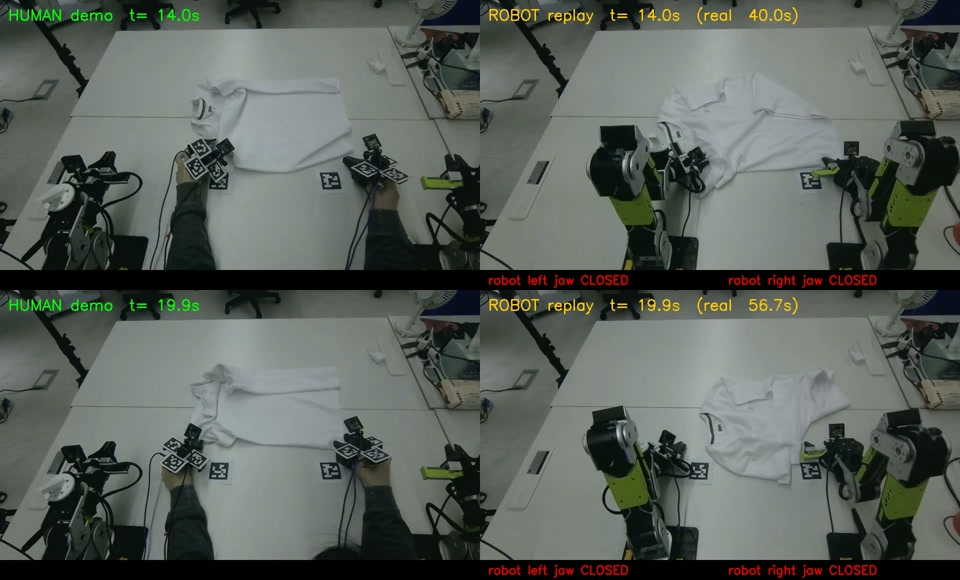
\includegraphics[width=0.85\textwidth]{figures/fig_sidebyside.jpg}
\caption{사람 시연(왼쪽)과 변환된 궤적의 양팔 로봇 재생(오른쪽). 같은 고정 카메라로 촬영하고 하나의 시계로 맞췄다(로봇
0.35$\times$). 막대는 로봇 집게 명령이다. 집게가 셔츠 가장자리를 잡아 끌며, 셔츠는 움직였지만 사람처럼 개지지는 않았다.}
\label{fig:sbs}
\end{figure*}

\textbf{전체 시연의 양팔 재생.} 33\,s 시연 하나를 사람 속도의 약 3분의 1로 재생했다(94\,s; 그림~\ref{fig:sbs}). 그 구간에서
오른손은 프레임의 79\,\%, 왼손은 95\,\%에서 마커가 보였고, 오른손 프레임의 21\,\%는 보간되었다. 로봇화 변위의 p95는 9.3\mm(오른손),
20.6\mm(왼손)였다. 계획은 IK 오차를 6.3\mm / 11.5$^\circ$(오른쪽), 10.3\mm / 21$^\circ$(왼쪽) 이내로 유지했고, 두 팔은 적어도
27\,cm 떨어져 있었다. 표~\ref{tab:rep}는 같은 계획으로 한 네 번의 실행 오차를, 재생한 로봇화 경로를 기준으로 보인다. 실행 간 차이는
약 1\mm{}이다. 로봇은 결정적이며 남은 오차는 계통적이다. 원래 사람 경로 기준 RMSE는 약 22\mm(오른쪽), 32--34\mm(왼쪽)인데, 이때는
로봇화 변위도 오차로 세기 때문이다. 왼쪽 명령은 이미 재생 경로에서 더 벗어난다(B$-$A 22.6\mm 대 8.6\mm). 왼쪽 IK가 방향을 더
포기하기 때문이다.

\begin{table}[t]
\caption{양팔 재생, 같은 계획으로 한 네 번 실행의 범위(시연 전체가 한 창; 기준 = 로봇화 경로)}\label{tab:rep}
\centering\small
\begin{tabular}{@{}lcc@{}}
\toprule
 & 오른쪽 & 왼쪽 \\
\midrule
위치 RMSE & 17.2--17.4\mm & 29.0--30.3\mm \\
위치 p95 & 35--37\mm & 50--51\mm \\
회전 중앙값 & 8.1$^\circ$ & 12.3--12.7$^\circ$ \\
회전 p95 & 12.6--12.7$^\circ$ & 17.0--17.2$^\circ$ \\
C$-$B(추적) & 12.1--12.3\mm & 14.5--15.5\mm \\
B$-$A(변환, IK) & 8.6\mm & 22.6\mm \\
\bottomrule
\end{tabular}
\end{table}

\textbf{잡을 때의 집게 높이.} 보수적인 손가락 모서리 여유로는 집게가 테이블 위 19--61\mm{}에서 닫혀 천을 놓쳤다. 사람 손가락처럼
손가락 모서리가 테이블 평면에 닿도록 허용하자 닫히는 높이가 14--16\mm(오른쪽, 4회), 5--19\mm(왼쪽, 5회)가 되었고, 그 순간 명령과의
$xy$ 차이는 2--8\mm{}였다. 사람은 약 10\mm{}에서 닫는다(그림~\ref{fig:close}). 대신 공구를 수직 쪽으로 기울이는 방법은 실패했고(IK가
15$^\circ$도 따라가지 못해 오차가 최대 100\mm), 근처의 가장 낮은 점에서 닫는 휴리스틱은 기각했다.

\begin{figure}[!t]
\centering
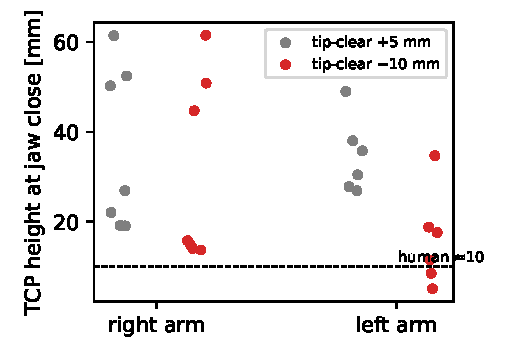
\includegraphics[width=0.62\columnwidth]{figures/fig_close_height.pdf}
\caption{보수적인 손가락 모서리 여유와, 모서리가 테이블 평면에 닿도록 허용했을 때의 집게 닫힘 순간 TCP 높이. 점선: 사람
($\approx$10\mm).}
\label{fig:close}
\end{figure}

\textbf{결과.} 두 번의 실행에서는 셔츠가 시연보다 15--20\,cm 멀리 놓여 집게가 빈 테이블에서 닫혔다. 한 번은 집게가 셔츠 가장자리를
잡아 끌었다. 셔츠는 움직였지만 사람처럼 개지지 않았다. 개루프 재생은 천이 사람의 것과 같은 자리에 있어야 하므로, 다음 단계는
천을 보는 정책이다.

% =====================================================================
\section{정책 학습 데이터}\label{sec:data}
\textbf{수집.} 구겨진 티셔츠를 \emph{펴는} 시연 318개를 10월 26일과 27일에 녹화했고, 300개가 성공했다(베이지 72, 검정 92, 흰색 82,
파랑 54). 성공 여부는 각 시연이 끝나기 0.5\,s 전 프레임으로 판정했다. 양손이 화면 안에 있도록 카메라는 113\,cm에 있다. 10월 22일과
그 이후 테이크에서 리그 라벨이 손목 카메라와 뒤바뀐 것이 발견되어, 각 그리퍼 궤적은 테이블의 어느 쪽에 있는지로 팔에 배정한다.

\textbf{트림.} 기다리는 시작과 멈춘 끝은 동작으로 학습될 수 있다. 각 시연은 어느 한 손이 10\,cm/s보다 빠르게 움직이는 첫 순간
0.3\,s 전부터 마지막 순간 0.3\,s 후까지로 자른다. 창 시작 0.5\,s 안에서 시작하는(또는 끝 0.5\,s 안에서 끝나는) 0.8\,s 이상의 한 손
추적 공백은, 남는 길이가 8\,s 미만이 되지 않는 한 등급을 낮추지 않고 잘라 낸다.

\textbf{등급.} 두 팔 모두 커버리지 $\ge$0.95, 1\,s 넘는 공백 없음, 보이는 마커에서 10\,cm 넘게 떨어진 유효 프레임 비율 0.05 이하,
그런 연속 구간 0.5\,s 이하, 손 바뀜 프레임 없음, 첫 1초 정상, 집게 이벤트 $\pm$1\,s 안에 1\,s 이상 공백 없음이면 \textbf{GOLD};
어느 팔이든 3\,s 넘는 공백, 커버리지 0.80 미만, 멀리 벗어난 프레임 0.20 초과, 2\,s 넘는 연속 구간, 1\,s 넘는 손 바뀜이 있으면
\textbf{REJECT}; 나머지는 \textbf{SILVER}. 시연은 통째로 남기거나 버린다. 처음 등급을 매긴 139개 중 133개가 GOLD, 5개가 SILVER,
1개가 REJECT이다. 펴기 파인튜닝에는 300개 전체에서 고른 GOLD 시연 281개를 쓰며, 300개 전체의 최종 등급 수는 여기서
보고하지 않는다.

\textbf{IK 이전 라벨.} 이전 라벨 B는 로봇화 경로의 IK$\to$FK였다. IK는 실행상의 선택(손목 롤 완화, 관절 한계 근처의 180$^\circ$
공구 뒤집기, 두 팔을 떼어 놓는 밀어내기)을 하고 이를 데이터에 굳히며, 바로 중요한 곳에서 목표를 가장 많이 옮겼다. 처음 139개
시연(약 123k 팔-프레임)에서 IK$\to$FK는 목표를 전체 p95 $\approx$53\mm, 잡는 순간 $\approx$58\mm 옮긴다(표~\ref{tab:ikqa}). 같은
시연에서 20.3\,\%의 프레임은 큰 IK 보정이 필요하며 대부분 실행상의 선택 때문이고, 정말 닿을 수 없는 프레임은 0.8\,\%이다(손을
테이블 위로 높이 든 경우). 그래서 라벨은 IK 이전의 데카르트 집게 끝 자세이며 $B$에 절대값으로 저장한다. IK는 오프라인에서는
검사기, 온라인에서는 실행기이고, B는 QA용으로만 남긴다. 라벨 F와 A에서 IK 결과는 값을 바꾸지도 프레임을 mask하지도 않으며, IK를
아예 돌릴 수 없는 시연만 빠진다.

\begin{table}[t]
\caption{데카르트 라벨의 IK 검사(처음 139개 시연). ``큰 보정'' = IK 위치 오차 $>$30\mm 또는 회전 $>$30$^\circ$; 원인은 순서대로
배정하며 처음 맞는 것을 택한다.}\label{tab:ikqa}
\centering\small
\begin{tabular}{@{}lccc@{}}
\toprule
 & 전체 & 왼쪽 & 오른쪽 \\
\midrule
IK$\to$FK 대 데카르트, 위치 p95 & 53\mm & 70\mm & 28\mm \\
큰 보정이 필요한 프레임 & 20.3\,\% & 27.8\,\% & 12.9\,\% \\
\quad 손목 롤 완화 & 7.6\,\% & 14.8\,\% & 0.4\,\% \\
\quad 기타(IK 지연) & 4.1\,\% & 5.9\,\% & 2.3\,\% \\
\quad 관절 한계 & 3.2\,\% & 2.9\,\% & 3.5\,\% \\
\quad 공구 뒤집기 & 3.1\,\% & 1.3\,\% & 4.9\,\% \\
\quad 작업 공간 / 테이블 & 0.8\,\% & 0.9\,\% & 0.7\,\% \\
\quad 도달 불가 & 0.8\,\% & 1.3\,\% & 0.4\,\% \\
\quad 팔 간격 & 0.6\,\% & 0.6\,\% & 0.6\,\% \\
\bottomrule
\end{tabular}
\end{table}

\textbf{라벨 F: 클램프 없음(10월 29일).} 라벨 A는 reBot 집게 축으로 나타낸 융합 집게 끝 자세를 0.25\,s로 평활하고, 테이블 여유
단계(수직 쪽으로 최대 30$^\circ$ 기울인 뒤 손가락 모서리 들어 올림)를 더한 것이다. 이 단계가 라벨 프레임의 44\,\%를 중앙값
27\mm(최대 65\mm) 들어 올려서, 정책은 천까지 내려가는 법을 배울 수 없었다(\ref{sec:policy}절). 현재 라벨 F는 여유 단계를 뺀 같은
자세다. 0.25\,s 평활은 그대로이고 클램프, 들어 올림, 실현 가능성 편집이 없으며, IK는 값을 바꾸지도 mask하지도 않는다. 한계는 학습 라벨이 아니라 배포의 몫이다.

\textbf{시간 늘이기.} 사람 시연은 팔이 따라갈 수 있는 것보다 빠르다(집게 끝 p95 0.93\,m/s, 127$^\circ$/s). 시간을 늘린 데이터
사본은 자세, 집게 이벤트, 모든 카메라 프레임(가장 가까운 원본 프레임)을 하나의 더 느린 공통 시간축으로 다시 샘플링한다. 배율 $s$에서
행은 20\,Hz 그대로이고 원본 시간으로 $s\cdot$0.05\,s씩 나아가므로 시연이 $1/s$배 길어진다. 펴기 세트는 0.3$\times$, 집기 세트는
0.5$\times$이다.

\textbf{데이터셋.} LeRobot v3, 20\,Hz, 카메라 셋(고정 카메라와 두 손목 카메라), 30-D 상태(팔마다 에피소드 시작 기준 상대 자세,
두 집게, 좌우 상대 자세), 20-D 절대 액션(팔마다 위치와 6-D 회전, 그다음 두 집게; 집게 목표는 0.1\,s 램프를 둔 이진 집게 상태)과
차원별 마스크. 정책은 학습 로더에서 만드는 상대 동작 $T_t^{-1}T_{t+k}$, $k=1\ldots32$를 배운다.

% =====================================================================
\section{로봇에서의 첫 정책}\label{sec:policy}
\textbf{배포 루프.} 매 주기 새 영상과 측정 관절을 받고, FK로 현재 TCP를 얻고, 정책이 상대 스텝 32개를 예측하고, 가장 최근 TCP로
청크를 다시 고정하고(지연), 제한기가 속도와 테이블 바닥을 제한하고, Pink IK가 관절을 풀고, 안전 검사(작업 공간, 링크 간 캡슐,
테이블, 관절 한계)를 통과해야 한다. 재계획 전에는 계획의 앞 스텝만 실행한다(DiT 기본값 4; 그림~\ref{fig:deploy}). 10월 27일 집게 열림
한계 없이 브리지를 재시작하자 한 집게가 끝까지 열려 홀더가 부러졌다. 이제 배포는 브리지가 집게 한계를 보고하지 않으면 명령을
보내지 않는다.

\begin{figure}[!t]
\centering
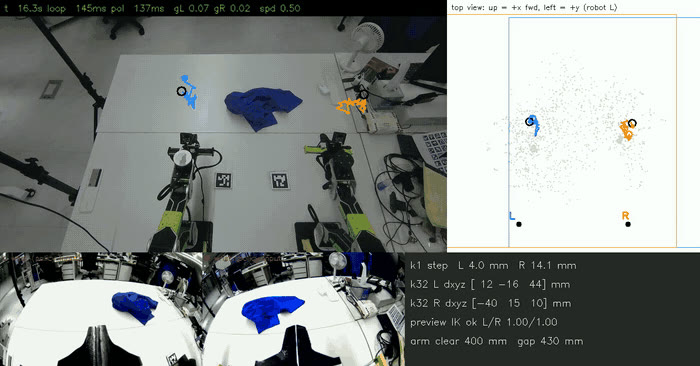
\includegraphics[width=\columnwidth]{figures/fig_deploy_ui.jpg}
\caption{드라이 런(명령을 보내지 않음) 중의 배포 UI: 고정 카메라 위에 예측한 32 스텝 집게 끝 경로(왼쪽 파랑, 오른쪽 주황), 로봇
베이스 기준 위에서 본 모습, 두 로봇 손목 카메라, 실시간 검사.}
\label{fig:deploy}
\end{figure}

\textbf{정책.} (1) 공개 천 개기 데이터 Soft-Fold로 300k 스텝 사전학습한 디퓨전 트랜스포머 정책(DiT, CLIP~\cite{radford2021clip}
텍스트, 관측 프레임 2개, 호라이즌 33)은 로봇에서 드라이 런으로 안전 위반 없이 동작했다. 우리 데이터의 DiT 파인튜닝은 Soft-Fold,
iPhUMI~\cite{iphumi}, PrimeBot UMI~\cite{primebot}를 1\,:\,1\,:\,1로 섞어 100k 스텝 사전학습한 DiT에서 시작한다. (2) 같은 세 데이터를
1\,:\,1\,:\,1로 섞어 사전학습한 X-VLA 기본 모델~\cite{xvla}, 소스마다 도메인 프롬프트 하나. 둘 다 GOLD 펴기 시연 281개로
파인튜닝했고(10월 말부터), 후퇴 호라이즌 루프로 실행했다. 이 실행에서 알려진 것은 정성적인 관찰이다. 팔은 천 쪽으로 가지만 닿기
전에 멈추고 집게를 일찍 닫았다. 시행 횟수는 세지 않았고, 10월 28--31일 실행의 체크포인트, 라벨 종류, 속도는 기록되지 않았다.
\textbf{성공률은 보고하지 않는다.}

\textbf{원인과 데이터 문제.} 로봇 실행에서 기록된 원인은 집게 상태 따라 하기와 손목 카메라 위치 두 가지다(표~\ref{tab:causes}의
첫 행과 마지막 행). 나머지 세 행은 그 뒤 라벨을 점검해 찾았다. 카메라 재장착을 빼고 모두 바꾸었고, 다음은 로봇 손목 카메라
재장착이다.

\begin{table}[t]
\caption{첫 정책들이 드러낸 데이터 문제(10월 28일 -- 11월 1일)}\label{tab:causes}
\centering\small
\begin{tabular}{@{}>{\raggedright\arraybackslash}p{0.45\columnwidth}>{\raggedright\arraybackslash}p{0.47\columnwidth}@{}}
\toprule
발견 & 변경 \\
\midrule
집게가 일찍 닫히고 다시 열리지 않음: 정책이 관측 입력의 집게 상태를 그대로 따라 함 & 학습과 배포에서 관측의 집게 상태를 0으로 가림 \\
라벨의 테이블 여유가 프레임 44\,\%를 27\mm(중앙값) 들어 올림 & 라벨 F: 융합 집게 끝, 클램프 없음(\ref{sec:data}절) \\
시연이 팔보다 빠름(p95 0.93\,m/s, 127$^\circ$/s) & 시간을 늘린 사본, 0.3$\times$ / 0.5$\times$ \\
영상 집게 라벨이 실제 열림과 다름 & 10월 29일부터 서보 엔코더 라벨; 섞지 않음(\ref{sec:jaw}절) \\
로봇 손목 카메라가 손 착용 카메라보다 공구 축 쪽으로 11--13$^\circ$ 덜 기울고 25--44\mm 더 가까움(테이블 태그 PnP) & 손 착용
형상에 맞춰 재장착(다음 단계) \\
\bottomrule
\end{tabular}
\end{table}

또한 추가했지만 \emph{아직 로봇에서 검증하지 않은} 것: 계획 사이의 실시간 청킹 블렌드(10월 29일부터 UI 기본값이지만 각 로봇 실행에서 켜져 있었는지는 기록되지 않음)와 X-VLA 정책 서버.

% =====================================================================
\section{집기 실현 가능성 시험(첫 로봇 잡기)}\label{sec:pinch}
``파이프라인이 잡기를 가르칠 수 없다''와 ``이 정도 데이터로는 펴기가 너무 어렵다''를 구분하려고, 첫 로봇 실현 가능성 시험을 하위
기술 하나로 줄였다: \textbf{왼손으로 소매 하나 집기}. 모든 데이터에서 오른팔은 움직이지 않는다. 11월 2일 로봇 실행에서는 두 팔 모두 정책이 제어했고 오른팔은
시작 자세에 머물렀다.

\begin{figure*}[!t]
\centering
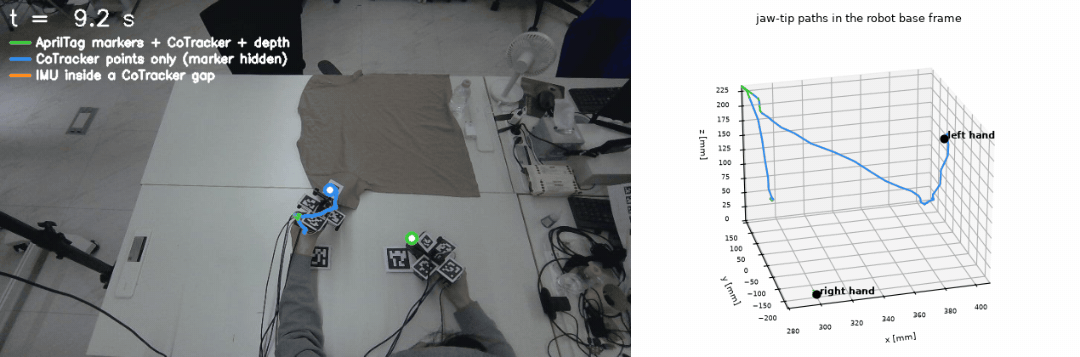
\includegraphics[width=0.85\textwidth]{figures/fig_pinching_cg.png}
\caption{11월 1일에 녹화한 GOLD 집기 시연: 프레임별 출처로 색칠한 Cg 집게 끝 경로(초록: 그리퍼 마커가 보임; 파랑: 마커가 가려져
점 추적만; 주황: 추적 공백 안의 IMU). 왼쪽: 고정 카메라에 투영; 오른쪽: 로봇 베이스 좌표계의 두 손. 오른손은 시작점 마커에
머문다.}
\label{fig:pinch}
\end{figure*}

\textbf{데이터.} 모든 세트가 Cg 궤적 소스(그림~\ref{fig:pinch})와 라벨 F, 서보 집게 라벨, 0.5$\times$ 시간 늘이기를 쓰며, GOLD와
SILVER 시연을 남긴다(표~\ref{tab:pinch}). 이전 궤적 소스(A$'$, 시연·팔마다 첫 2\,s의 태그로 구한 위치 편향 하나)는 11월 1일 일부
시연 안쪽에 NaN 구간이 있었고 그중 4개에서 IK가 실패해, 모든 세트를 Cg로 다시 만들었다. 두 소스는 섞지 않는다. 11월 1일에는 품질
게이트가 147개를 남겼고, 데이터셋 변환에서 trim 후 구간이 5\,s보다 짧은 3개가 빠져 10월 30일의 53개와 합친 학습 세트는 시연
197개(53 + 144, 62,160 프레임)이다.

\begin{table}[t]
\caption{집기 데이터, 11월 1일 기준(남김 = GOLD 또는 SILVER; 생성 = 데이터셋의 에피소드)}\label{tab:pinch}
\centering\small
\begin{tabular}{@{}lcccc@{}}
\toprule
녹화일 & 테이크 & 시연 & 남김 & 생성 \\
\midrule
10월 30일 & 5 & 74 & 53 & 53 \\
11월 1일, T1 + T2 & 2 & 60 & 56 & 55 \\
11월 1일, T3 & 1 & 35 & 33 & 33 \\
11월 1일, T4 & 1 & 10 & 10 & 10 \\
11월 1일, T5 & 1 & 50 & 48 & 46 \\
\bottomrule
\end{tabular}
\end{table}

\textbf{시험 세트(학습에 쓰지 않음).} P20: held-out 테이크 두 개에서 나온 시연 19개(6207 프레임), 팔과 집게용. 10월 30일 테이크의
시연 10개 전부(게이트로 거르지 않음)와 11월 1일 테이크의 10개 중 9개(열 번째는 기각). 기각 세트: 11월 1일 시연 중 품질 게이트가 기각한 모든 시연으로, 서보 집게
라벨은 유효하고 팔 라벨은 그렇지 않으므로 집게 타이밍에만 쓴다.

\textbf{모델.} 10월 30일 시연 53개(궤적 소스 A$'$, 라벨 F)로 파인튜닝한 DiT가 출발점이자 기준선이다. Cg로 만든 P20에서 19.89\mm{}를
기록한다(\code{val_score_mm}: $k=16$과 $k=32$, 왼팔과 오른팔에 걸친 이동 편차의 평균, 위치만; 소스 A$'$로 만든 P20에서는 19.13\mm). P10의 시연 10개에서의 점수는
약 150 에포크 이후 17.1--17.7\mm{}에서 정체했다. 이 가중치에서 시작해 합친 Cg 시연 197개로 새 옵티마이저와 500 에포크 코사인 스케줄,
25 에포크마다 체크포인트, 그래디언트 클리핑 없음, 집게 BCE 헤드, 새 학습 시 이미지 증강으로 하는 파인튜닝을 11월 1일에 시작했으며(약
4.7일 예정). P20에서 25 에포크와 50 에포크 체크포인트는 각각 17.29\mm{}와 18.89\mm{}를 기록했다(기준선 19.89\mm).
로봇에서 잡은 것은 50 에포크 체크포인트이므로, 오프라인 점수가 로봇용 체크포인트를 골라 주지는 못했다. 이 사슬의 앞 단계에서는 세 데이터 혼합으로 사전학습한 DiT를 펴기 GOLD 시연(라벨 F, 0.3$\times$)으로,
이어서 집기 데이터로 파인튜닝한 뒤 10월 30일 세트로 넘어왔다.

\textbf{로봇 쪽 변경.} 테이블 태그를 집게 끝으로 짚어 팔마다 테이블 높이를 캘리브레이션하고(평면 기울기 왼쪽 4.9$^\circ$, 오른쪽
2.6$^\circ$) UI 옵션을 켜면 실행하는 모든 명령에 더함; 10월 26일 이후 움직인 고정 카메라를 이전 시야로 다시 맞춤(잔차 약 5\,px / 0.4$^\circ$);
비상 정지를 걸지 않고 현재 명령에서 감속하는 부드러운 정지.

\textbf{11월 1일 로봇 실행(정성 관찰, 횟수 세지 않음).} DiT 체크포인트 두 개를 계획당 32 스텝 실행, 속도 1(나중에 1.5)로 돌렸다.
GOLD 281개 + 서보 라벨 시연 48개로 파인튜닝한 펴기 정책(라벨 F, 0.3$\times$; 약 70\,s 실행 두 번)과 집기 기준선(짧은 실행 한 번)이다.
둘 다 왼쪽 집게는 대부분 열림 명령이었고 오른쪽 집게는 닫힌 채였다. 첫 실행에서 왼쪽 손목 모터 오류가 한 번, 왼팔이 명령보다
20$^\circ$ 넘게 뒤처진 적이 한 번 있었다. 성공이나 실패는 매기지 않았다.

\begin{figure*}[!t]
\centering
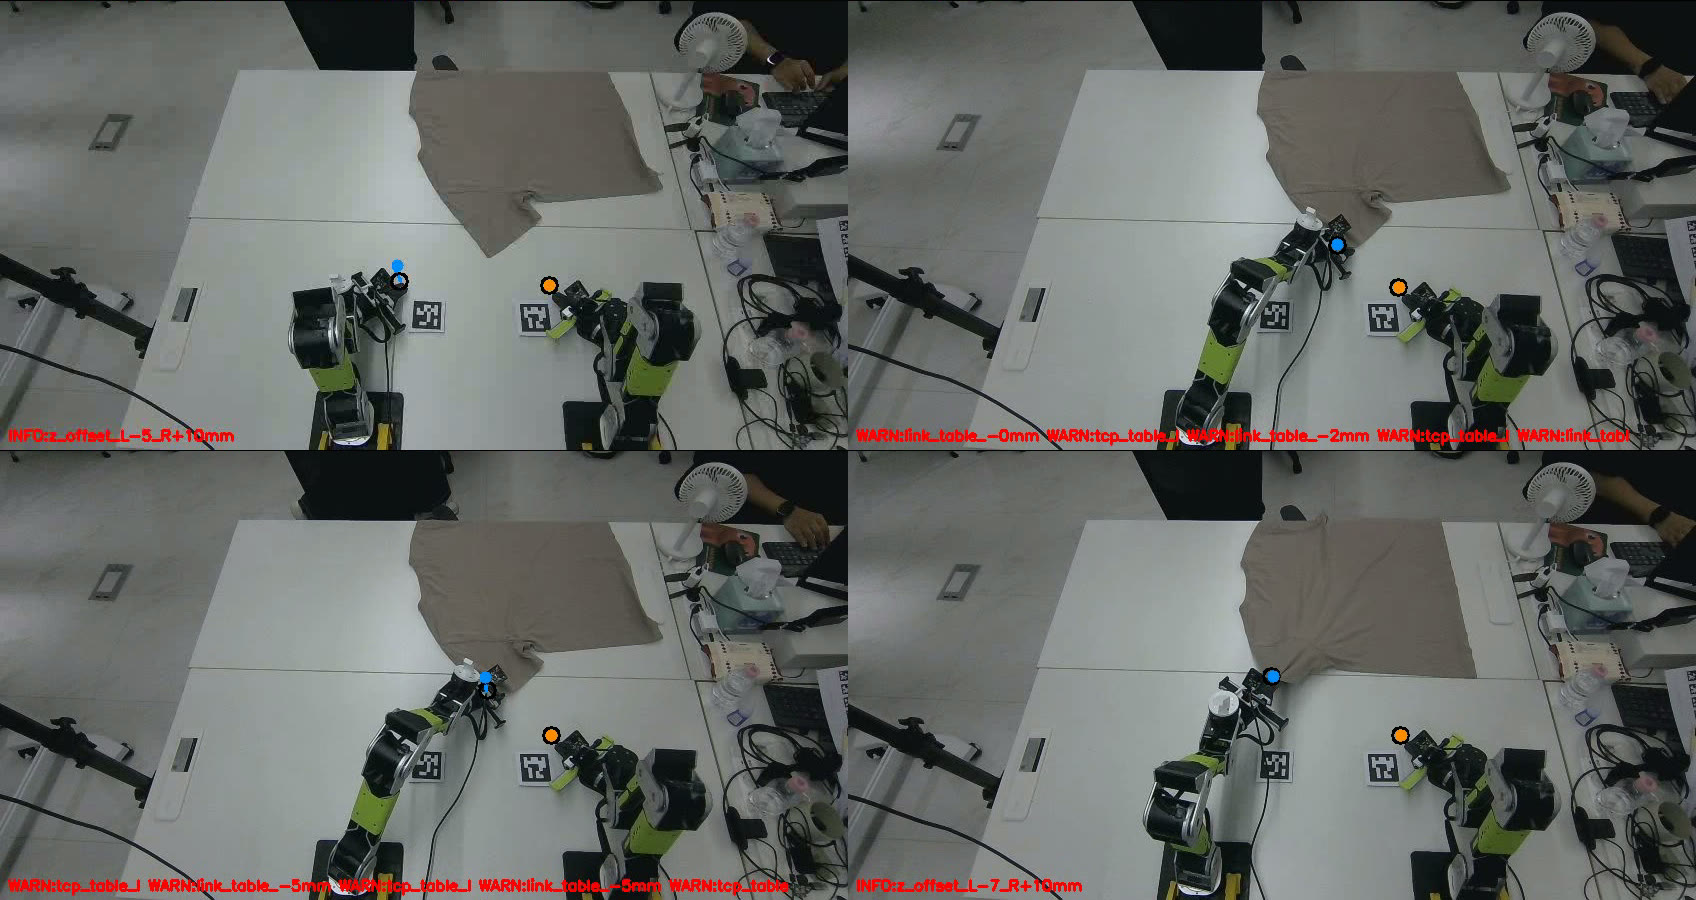
\includegraphics[width=0.85\textwidth]{figures/fig_pinching_robot_1102.jpg}
\caption{11월 2일 실제 로봇 실행 중 운영자가 성공으로 판단한 한 실행(50 에포크 체크포인트; 고정 카메라, 계획 주기마다 한 프레임;
시행 횟수는 세지 않음). 왼쪽 위: 시작; 오른쪽 위: 왼팔이 집게를 연 채 소매 끝으로 접근(7\,s); 왼쪽 아래: 소매에서 집게를 닫음(11\,s);
오른쪽 아래: 소매를 당김(22\,s). 파란/주황 점: 왼쪽/오른쪽 집게에 대한 정책의 다음 목표. 빨간 글씨: 배포 루프의 테이블 근접 메시지.}
\label{fig:pinchrobot}
\end{figure*}

\textbf{11월 2일 로봇 실행(첫 잡기; 시행 횟수는 세지 않음).} 197개 시연 파인튜닝의 50 에포크 체크포인트를 계획당 32 스텝 실행, 속도 1,
실시간 청킹 look-ahead 끔, DDIM 샘플링 10 스텝, 팔별 높이 캘리브레이션 켬, 부드러운 정지로 돌렸다. 11월 2일 실제 로봇 시행에서
소매를 잡는 데 성공하는 것이 관찰되었다(그림~\ref{fig:pinchrobot}): 왼팔이 집게를 연 채 소매 끝으로 가서 닫고 당긴다. 시행 횟수는
세지 않았으므로 성공률은 제시하지 않는다. 놓친 뒤에는 정책이 다시 시도하지 않고 다른 곳을 잡는다. 데이터에 복구 시연이 없어 실패
이후의 상태가 분포 밖이기 때문이다. 다시 하려면 팔을 시작 자세로 돌려 처음부터 시작한다. 데이터 쪽 해결책은 복구 시연을 녹화하는
것이다. 그날의 하드웨어 변경: 재배선 뒤 두 팔의 USB 위치가 뒤바뀌어 실행 설정에서 고침; 왼쪽 집게에 기계적 유격이 생겨 이제 영점보다
25$^\circ$ 더 닫으며, 추가로 조이는 양은 닫히기 전 마지막 30$^\circ$ 구간에서만 점차 더함; 시작 자세로 갈 때 두 집게를 모두 닫음(토크를
끈 집게는 저절로 벌어짐); 로봇 손목 카메라 하나가 한 번 멈춰 배포 UI를 다시 시작함.

\textbf{현황: 첫 잡기 관찰, 시행 횟수는 세지 않음.} 로봇 시행은 결과와 관계없이 시행 횟수와 성공 횟수로 보고할 것이다.

% =====================================================================
\section{대체된 방법}\label{sec:superseded}
\begin{table*}[t]
\caption{현재 파이프라인과 그것이 대체한 것}\label{tab:superseded}
\centering\small
\begin{tabular}{@{}>{\raggedright\arraybackslash}p{0.11\textwidth}>{\raggedright\arraybackslash}p{0.36\textwidth}>{\raggedright\arraybackslash}p{0.30\textwidth}>{\raggedright\arraybackslash}p{0.16\textwidth}@{}}
\toprule
부분 & 현재(11월 1일) & 대체된 것 & 이유 \\
\midrule
자세 소스 & 고정 카메라 CoTracker3 + 마커 앵커 + 일정 편향, 공백에서만 IMU(Cg) & MASt3R 손목 SLAM 공백 채우기; ORB-SLAM3;
스테레오 VIO; SLAM + 몸체 추적 평활기; 마커 + IMU 채움(재생 트랙) & 잡을 때 잃음; 스케일 관측 불가; 라벨 오차 4--6\,cm \\
카메라 $\leftrightarrow$ 로봇 & 카메라를 옮길 때마다 테이블 태그 두 장 + 테이블 평면으로 다시 풀이 & 로봇이 든 마커로 한 32개 자세 풀이 &
양손이 화면 안에 있도록 카메라를 올림 \\
집게 상태 & 서보 엔코더(10월 29일부터); 이전 시연은 영상 모델 & 빨간 테이프 집게 검출기(10월 20일 테이프 제거) & 검출기가 배경에
반응; 영상 라벨이 서보와 불일치 \\
팔 배정 & 그리퍼가 테이블의 어느 쪽에 있는지 & 리그 라벨 & 라벨이 뒤바뀜 \\
라벨 & F: IK 이전의 융합 집게 끝(집게 축, 0.25\,s 평활), 클램프 없음 & B: IK$\to$FK; A: 테이블 여유 포함 & IK 선택과 클램프가 잡는 순간 목표를 옮김 \\
데이터 속도 & 0.3$\times$ / 0.5$\times$로 늘린 사본 & 사람 속도 & 팔에 너무 빠름 \\
실행 & 후퇴 호라이즌 배포, 계획당 4 스텝(DiT 기본값) & 시연 전체 개루프 재생 & 재생은 같은 장면이 필요 \\
\bottomrule
\end{tabular}
\end{table*}

표~\ref{tab:superseded}는 무엇이 대체되었는지, 현재 파이프라인이 언제 만들어졌는지, 그리고 그 이유를 정리한다. 버린 방법의 코드는
날짜와 이유를 정리한 README 표와 함께 \code{legacy/}에 있다.

% =====================================================================
\section{교훈}\label{sec:lessons}
\begin{enumerate}
\item \emph{접촉이 많은 손 동작에서는 마커와 고정 카메라가 손목 SLAM보다 낫다.} SLAM의 실패 조건(가까운 거리, 질감 없는 천, 빠른
  동작)이 바로 잡는 순간이다.
\item \emph{대체하지 말고 고정하라.} 점 추적이 가려진 구간을 덮고, 마커가 그 절대 오차를 없앤다. 어느 하나만으로는 부족하다.
\item \emph{모델이 아니라 현실에서 재라.} 89\mm TCP 오차와 70\mm 베이스 오차는 FK 기반 검사로 보이지 않았고, 줄자·카메라·천이 찾아냈다.
  이전 평활기의 4--6\,cm 오차는 자체 잔차로 보이지 않았다.
\item \emph{휴리스틱을 더하지 말고 변환을 고쳐라.} 여유를 위해 집게를 들어 올리자 잡기를 잃었고, 접촉을 허용하자 되찾았다.
\item \emph{실행기나 안전 한계가 라벨을 쓰게 하지 마라.} IK 선택과 테이블 클램프는 실행에는 옳고 학습 목표로는 틀리다.
\item \emph{모든 것에 하나의 시계.} 동기화 하드웨어 없이 카메라·IMU·서보·로봇 정렬과 나란히 보기 영상을 가능하게 했다.
\item \emph{제어기를 모델링하라.} 추적 오차는 $\dot\tau_g/K_i$를 따랐고, $K_p$를 바꿔서는 도움이 되지 않았다.
\end{enumerate}

% =====================================================================
\section{한계}\label{sec:limits}
\begin{itemize}
\item \emph{성공률 없음.} 재생도 정책도 횟수를 센 시행으로 돌리지 않았으며, 결과는 측정과 영상으로 판단했다.
\item \emph{셋업 하나, 시연자 한 명.} 모든 숫자는 물리 셋업 하나와 한 사람에게서 나왔다. 양팔로 전체를 재생한 시연은 하나이며,
  1\mm 반복성은 결정성을 보일 뿐 일반성을 보이지 않는다.
\item \emph{상대 일치도 지표는 오프셋을 숨긴다.} 절대 위치는 몇 자세에서의 줄자와 영상으로만 확인했다.
\item \emph{잡는 순간의 자세 정확도.} 가린 마커 오차는 마커를 가릴 수 있는 곳, 대개 잡는 순간에서 떨어진 곳에서 잰다. 긴 추적 공백
  안의 오차는 게이트로만 제한된다.
\item \emph{여기 보고한 등급과 IK 통계}는 처음 139개 펴기 시연에서 계산했고, 300개 전체의 최종 등급 수는 보고하지 않으며, 성공 여부는 한 사람이 프레임 하나로 판정했다.
\item \emph{손목 영상의 집게 라벨}은 이전 시연에서 held-out 정확도 수치가 없고, 둘 다 있는 곳에서 서보와 프레임의 약 70--80\,\%에서만
  일치한다.
\item \emph{오프라인 점수}(\code{val_score_mm} 등)는 held-out 사람 동작과의 일치를 재며, 과제 성공을 재지 않는다.
\item \emph{하드웨어.} 왼쪽 로봇 손목 커넥터가 여러 번 끊겼다.
\end{itemize}

% =====================================================================
\section{재현성}\label{sec:repro}
\textbf{저장소 구성.} \code{src/garment_pipeline/}: 설치 가능한 패키지로서의 학습 데이터 파이프라인(융합, 게이트, 트림, 등급, 라벨,
LeRobot 데이터셋, DiT 학습기, 오프라인 평가, 배포), \code{python -m garment_pipeline.<stage>.<module>}로 실행;
\code{src/visual_teleop/}: 녹화기, 집게 분류기, reBot IK, 한계, 안전, 재생 계획기; \code{src/rebot_prep/}: 공유 마커 리그 자세 코드;
\code{scripts/pose/}, \code{scripts/retarget/}, \code{scripts/evaluation/}, \code{scripts/deploy/}: 캘리브레이션, 서보 집게 라벨,
재생용 로봇화, 일치도 채점, 로봇 브리지; \code{src/egogarment/}: \code{examples/}의 합성 데이터에서 도는 궤적 단계의 작은 독립
재구현; \code{configs/}: 캘리브레이션 결과와 로봇 덮어쓰기; \code{hardware/umihand/}: 우리 수정이 들어간 HandUMI 빌드 사본(업스트림
Apache-2.0 라이선스 유지); \code{legacy/}: 대체된 코드; \code{docs/}, \code{media/}, \code{report/}: 문서, 미디어, 이 보고서.

\textbf{포함하지 않은 것.} 원시 녹화, 학습된 체크포인트, reBot 제조사 플러그인과 URDF, ORB-SLAM3 소스, X-VLA 파인튜닝 코드. 실제
데이터 단계는 녹화가 필요하고, 일부는 GPU나 로봇이 필요하다.

\textbf{검증 방법.} 체크아웃에서 \code{pip install -e ".[test]"} 후 \code{python -m pytest -q}(합성 예제에서 독립 도구의 회귀, import와
설정 경로 스모크 테스트), \code{python scripts/evaluation/replay_parity.py --synthetic}과 \code{python scripts/pose/robot_cam_solve.py --synthetic}
(모의 데이터에서 일치도 채점기와 카메라--로봇 풀이기의 자체 시험)을 실행하며, 모두 CI에서 돈다. \code{python analysis/verify_claims.py}는
영문 보고서의 모든 숫자가 그것을 옮겨 온 저장소 안 문서(README, \code{docs/results.md}, \code{docs/details.md},
\code{docs/status_2026-11-01.md}, \code{docs/status_2026-11-02.md}, 보관한 보고서 v0.1)에도 있는지 확인한다. 이는 프로젝트 기록과의 일관성 검사이며, 데이터에서 숫자를
다시 계산하는 것은 아니다. 또한 한국어
보고서에 영문판에 없는 숫자가 없는지도 확인한다.

% =====================================================================
\section{결론과 다음 단계}\label{sec:next}
하나의 월드 좌표계와 하나의 시계로, 변환한 손 착용 그리퍼 시연은 양팔 로봇에서 결정적으로 재생되고 집게를 사람이 잡는 높이로
가져가며, 이는 캘리브레이션과 변환이 기하학적으로 타당함을 보인다. 개루프 재생으로 셔츠를 개지는 못한다. 고정 카메라 점 추적을
마커로 고정하는 자세 소스는 잡는 동안에도 집게 끝 자세를 유지하며, 학습 라벨은 이제 클램프 없이 IK 이전의 융합 집게 끝이고,
서보 집게 라벨과 느린 시간을 쓴다. 횟수를 세지 않은 로봇 시행에서 첫 정책들은 천에 닿기 전에 멈췄고, 기록된 원인과 그 뒤 찾은 라벨
문제는 카메라 재장착을 빼고 모두 바꾸었다. 범위를 줄인 집기 시험에서는 시연 197개로 파인튜닝한 정책이 11월 2일 횟수를 세지 않은
로봇 시행에서 소매를 잡았으며, 놓친 뒤에는 복구하지 못한다. 다음: 복구 시연을 녹화하고, 로봇 손목 카메라를 재장착하고, 횟수를 센 로봇 시행으로 집기 시험을 마친 뒤, 고친
라벨과 서보 라벨 시연으로 학습한 펴기 정책을 횟수를 센 시행으로 평가한다.

\section*{감사의 글}
손 착용 그리퍼는 BrikHMP18의 HandUMI(murobotics-ai, Apache-2.0)이며 UMI~\cite{chi2024umi}를 따른다. 사전학습 데이터: Soft-Fold,
iPhUMI(MIT), PrimeBot UMI(CC BY-SA 4.0).

\begin{thebibliography}{99}\footnotesize
\bibitem{chi2024umi} C.~Chi, Z.~Xu, C.~Pan, E.~Cousineau, B.~Burchfiel, S.~Feng, R.~Tedrake, and S.~Song, ``Universal
Manipulation Interface: In-the-wild robot teaching without in-the-wild robots,'' in \emph{Proc. Robotics: Science and Systems
(RSS)}, 2024. arXiv:2402.10329.
\bibitem{handumi} BrikHMP18 and murobotics-ai, ``HandUMI hardware (handumi-hw),'' GitHub repository, Apache-2.0, 2026.
\url{https://github.com/murobotics-ai/handumi-hw} (build copy from commit \texttt{e58de33}).
\bibitem{meza2026handumi} B.~Meza, L.~Perez, A.~Mendoza, A.~Ubillus, M.~Ramos, R.~Bastidas, M.~Olivera, and B.~Bastidas,
``HandUMI: A modular hand-worn parallel-jaw interface for robot-free bimanual data capture,'' 2026.
\url{https://murobotics.ai/research/handumi}
\bibitem{xu2025dexumi} M.~Xu, H.~Zhang, Y.~Hou, Z.~Xu, L.~Fan, M.~Veloso, and S.~Song, ``DexUMI: Using human hand as the
universal manipulation interface for dexterous manipulation,'' in \emph{Proc. Conf. Robot Learning (CoRL)}, 2025.
arXiv:2505.21864.
\bibitem{kareer2025egomimic} S.~Kareer, D.~Patel, R.~Punamiya, P.~Mathur, S.~Cheng, C.~Wang, J.~Hoffman, and D.~Xu,
``EgoMimic: Scaling imitation learning via egocentric video,'' in \emph{Proc. IEEE Int. Conf. Robotics and Automation
(ICRA)}, 2025. arXiv:2410.24221.
\bibitem{zhao2023aloha} T.~Z.~Zhao, V.~Kumar, S.~Levine, and C.~Finn, ``Learning fine-grained bimanual manipulation with
low-cost hardware,'' in \emph{Proc. Robotics: Science and Systems (RSS)}, 2023. arXiv:2304.13705.
\bibitem{cadene2024lerobot} R.~Cadene \emph{et al.}, ``LeRobot: State-of-the-art machine learning for real-world robotics in
PyTorch,'' 2024. \url{https://github.com/huggingface/lerobot}
\bibitem{avigal2022speedfolding} Y.~Avigal, L.~Berscheid, T.~Asfour, T.~Kr\"oger, and K.~Goldberg, ``SpeedFolding: Learning
efficient bimanual folding of garments,'' in \emph{Proc. IEEE/RSJ Int. Conf. Intelligent Robots and Systems (IROS)}, 2022.
arXiv:2208.10552.
\bibitem{ha2021flingbot} H.~Ha and S.~Song, ``FlingBot: The unreasonable effectiveness of dynamic manipulation for cloth
unfolding,'' in \emph{Proc. Conf. Robot Learning (CoRL)}, 2021. arXiv:2105.03655.
\bibitem{olson2011apriltag} E.~Olson, ``AprilTag: A robust and flexible visual fiducial system,'' in \emph{Proc. IEEE Int.
Conf. Robotics and Automation (ICRA)}, 2011.
\bibitem{wang2016apriltag2} J.~Wang and E.~Olson, ``AprilTag 2: Efficient and robust fiducial detection,'' in \emph{Proc.
IEEE/RSJ Int. Conf. Intelligent Robots and Systems (IROS)}, 2016.
\bibitem{bradski2000opencv} G.~Bradski, ``The OpenCV library,'' \emph{Dr.\ Dobb's Journal of Software Tools}, 2000.
\bibitem{collins2014ippe} T.~Collins and A.~Bartoli, ``Infinitesimal plane-based pose estimation,'' \emph{Int. J. Computer
Vision}, 2014.
\bibitem{terzakis2020sqpnp} G.~Terzakis and M.~Lourakis, ``A consistently fast and globally optimal solution to the
perspective-n-point problem,'' in \emph{Proc. European Conf. Computer Vision (ECCV)}, 2020.
\bibitem{karaev2024cotracker3} N.~Karaev, I.~Makarov, J.~Wang, N.~Neverova, A.~Vedaldi, and C.~Rupprecht, ``CoTracker3:
Simpler and better point tracking by pseudo-labelling real videos,'' 2024. arXiv:2410.11831.
\bibitem{mahony2008ahrs} R.~Mahony, T.~Hamel, and J.-M.~Pflimlin, ``Nonlinear complementary filters on the special
orthogonal group,'' \emph{IEEE Trans. Automatic Control}, 2008.
\bibitem{shah2013robotworld} M.~Shah, ``Solving the robot-world/hand-eye calibration problem using the Kronecker
product,'' \emph{J. Mechanisms and Robotics}, 2013.
\bibitem{pink} S.~Caron \emph{et al.}, ``Pink: Python inverse kinematics based on Pinocchio,'' software, Apache-2.0.
\url{https://github.com/pink-kinematics/pink}
\bibitem{carpentier2019pinocchio} J.~Carpentier, G.~Saurel, G.~Buondonno, J.~Mirabel, F.~Lamiraux, O.~Stasse, and
N.~Mansard, ``The Pinocchio C++ library,'' in \emph{Proc. IEEE/SICE Int. Symp. System Integration (SII)}, 2019.
\bibitem{murai2025mast3rslam} R.~Murai, E.~Dexheimer, and A.~J.~Davison, ``MASt3R-SLAM: Real-time dense SLAM with 3D
reconstruction priors,'' in \emph{Proc. IEEE/CVF Conf. Computer Vision and Pattern Recognition (CVPR)}, 2025.
\bibitem{campos2021orbslam3} C.~Campos, R.~Elvira, J.~J.~G\'omez~Rodr\'iguez, J.~M.~M.~Montiel, and J.~D.~Tard\'os,
``ORB-SLAM3: An accurate open-source library for visual, visual-inertial, and multimap SLAM,'' \emph{IEEE Trans. Robotics},
2021.
\bibitem{usenko2020basalt} V.~Usenko, N.~Demmel, D.~Schubert, J.~St\"uckler, and D.~Cremers, ``Visual-inertial mapping with
non-linear factor recovery,'' \emph{IEEE Robotics and Automation Letters}, 2020.
\bibitem{geneva2020openvins} P.~Geneva, K.~Eckenhoff, W.~Lee, Y.~Yang, and G.~Huang, ``OpenVINS: A research platform for
visual-inertial estimation,'' in \emph{Proc. IEEE Int. Conf. Robotics and Automation (ICRA)}, 2020.
\bibitem{xu2025airslam} K.~Xu, Y.~Hao, S.~Yuan, C.~Wang, and L.~Xie, ``AirSLAM: An efficient and illumination-robust
point-line visual SLAM system,'' \emph{IEEE Trans. Robotics}, 2025.
\bibitem{he2016resnet} K.~He, X.~Zhang, S.~Ren, and J.~Sun, ``Deep residual learning for image recognition,'' in
\emph{Proc. IEEE Conf. Computer Vision and Pattern Recognition (CVPR)}, 2016.
\bibitem{peebles2023dit} W.~Peebles and S.~Xie, ``Scalable diffusion models with transformers,'' in \emph{Proc. IEEE/CVF
Int. Conf. Computer Vision (ICCV)}, 2023.
\bibitem{radford2021clip} A.~Radford \emph{et al.}, ``Learning transferable visual models from natural language
supervision,'' in \emph{Proc. Int. Conf. Machine Learning (ICML)}, 2021.
\bibitem{xvla} X-VLA base model, \texttt{lerobot/xvla-base}, Hugging Face. \url{https://huggingface.co/lerobot/xvla-base}
\bibitem{iphumi} iPhUMI behavior-prompting data, \code{real-stanford/behavior_prompting}, Hugging Face, MIT licence.
\bibitem{primebot} PrimeBot challenge data, \code{challenge-2026/challenge_data}, Hugging Face, CC BY-SA 4.0.
\end{thebibliography}
\end{document}
